\section{\index{SiC!Silicon Carbide}{Silicon Carbide}}\label{SiC}

\index{SiC}{SiC} is a semiconductor which can be used for high-power and high temperature electronics \cite{Eddy2009,CASADY19961409}. Many studies have demonstrated SiC's potential as a host material for qubits, which enables the application of SiC quantum sensors even in ambient conditions \cite{PhysRevApplied.6.034001}. Moreover, 
the robustness of SiC allows for operation in extreme conditions
\cite{Cochrane2016}
.

\subsection{Colour Defects in SiC}
Point defects in wide-bandgap semiconductors can have both ground and excited states within the energy gap and, hence, are luminescent centres i.e. colour centres and the luminescence is often stable even at room temperature. 
Many color centers also possess a non-zero electron spin and can be excellent candidates for optical spin qubits \cite{Son2021}.

Recently, multiple colour centres have been observed in SiC, those which may be employed as spin qubits are the divacancy and the Silicon vacancy. 
There are seven types of divacancies in 4H-SiC, the polytope of SiC for which this work will be based. 
The defects can be categorised by their orientation within the lattice. 
These are the c-axis, for which we have the Silicon vacancy V2 and divacancies PL1, PL2, and PL6. 
On the basal axis, we have the divacancies PL3, PL4, PL5, and PL7 \cite{Qin-Yue}. 

Figure \ref{fig:SiC_defects} shows the position of the defects in the lattice. 

\begin{figure}[H]
    \begin{center}
        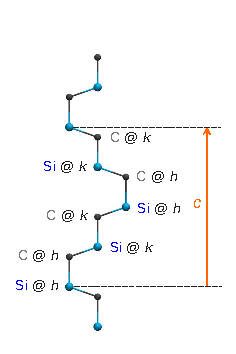
\includegraphics[width=0.32\textwidth]{figures/SiC-non-equiv-sites.pdf}
        \hspace{1em}
        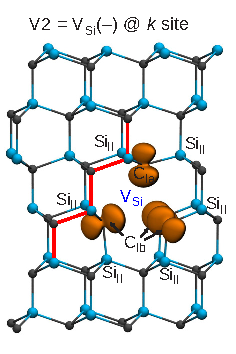
\includegraphics[width=0.32\textwidth]{figures/SiC-V2.pdf}
    \end{center}
    \caption{}\label{fig:SiC_defects}
    \todo[inline, color=ediblue]{Write caption and list source in et al format}
\end{figure}

Application of both the Silicon vacancy and the divacancies in quantum sensing can be competitive with the Nitrogen vacancy in diamond \cite{10.1093/nsr/nwab122}.


\subsection{Production of SiC}
Whilst the research for the Nitrogen vacancy in diamond is more mature, many equivalent techniques are being developed for 
SiC to compete with those which exist in diamond. 

Diamond is expensive and not compatible with conventional electronic circuits. By comparison, SiC is a technology-friendly material with an existing large-scale production capacity complemented by mature doping techniques \cite{Jiang2023}. Wafer-scale SiC is able to be produced and efficiently manufactured into electronic devices down to the atomic scale \cite{arxiv.1503.07566}.

Divacancies and Silicon vacancies may reliably introduced into SiC. As an example, the Silicon vacancy can be incorporated into the lattice and the density of the vacancies may be controlled down to the single defect level without degradation of the electrical characteristics of the material
\cite{Ohshima2018,PhysRevApplied.4.014009,Wang2019}
.

Further, approaches to manufacture solid-immersion lenses, which may aid the sensitivity or reduce the integration volume of a sensor have been demonstrated
\cite{Sardi2020}
.

Overall, research into the applicability of SiC as a quantum sensor is exciting and shows a lot of potential for application in the near term. 

% we discuss energetic particle irradiation, especially proton beam writing (PBW), in which proton microbeams with MeV range are used, as a method to create VSi in SiC since PBW can create VSi in certain locations with micrometer accuracy and this is very useful to introduce VSi in electronic devices without the degradation of their electrical characteristics.

% Interestingly, VSi can be incorpo-
% rated into SiC nanocrystals [28], and their density can be
% controlled over 8 orders of magnitude down to the single-
% defect level [32].

 % we present the generation and characterization of shallow silicon vacancies in silicon carbide by using different implanted ions and annealing conditions. 

% Here, we demonstrate a scalable approach of manufacturing solid-immersion lenses (SILs) on 4H–SiC.

